\documentclass{beamer}
\usetheme{CambridgeUS}
\usepackage{amsmath}
\usepackage{amsfonts}
\usepackage{amsthm}
\usepackage{amssymb}


\usepackage[utf8]{inputenc}


%Information to be included in the title page:
\title{Log-concave Sampling (Part 1)}
\author{Marios Papachristou}
\institute{GeomScale, NTUA}
\date{\today}

\begin{document}

\begin{frame}
    \titlepage
    \begin{center}
        
\includegraphics[width=0.3\textwidth]{publications/presentations/log_concave_sampling/logo.png} \quad 
        
\includegraphics[width=0.1\textwidth]{publications/presentations/log_concave_sampling/gsoc.png} 
    \end{center}
    
    \small {
    Mentors: A. Chalkis (NKUA), V. Fisikopoulos (NKUA), E. Tsigaridas (INRIA) \\
    Homepage: \url{https://github.com/GeomScale/volume_approximation}
    }
\end{frame}


\begin{frame}{About today's talk / tutorial}

Today's talk will concentrate on 
\\
\textbf{Sampling from high-dimensional log-concave densities}

\begin{enumerate}
    \item Main ideas 
    \item Un-Truncated Sampling
    \item Truncated Sampling
    \item Methods 
    \item Technical Implementations (for GSoC)
\end{enumerate}
    
\end{frame}

\begin{frame}{Google Summer of Code 2020}

The current GSoC project aims to provide implementations (and theoretical insights) to log-concave sampling problems for the GeomScale project.

Milestones 

\begin{enumerate}
    \item Milestone I (ODE Solvers)
    \begin{itemize}
        \item Implement ODE solvers (Euler, Runge-Kutta, Collocation, etc.)
        \item Efficiently address boundary oracles
    \end{itemize}
    \item Milestone II (Samplers) 
    \begin{itemize}
        \item Implement samplers (HMC, Langevin etc.).  
        \item Provide theoretical guarantees on truncated settings. 
    \end{itemize}
    
    \item Milestone III (R bindings)
    \begin{itemize}
        \item Port C++ functionality of 
    \end{itemize}
    
    
    Today's talk will mostly concentrate on \textbf{Milestone I}.
    
\end{enumerate}


    
\end{frame}

\begin{frame}{Basics}
    Our project involves taking samples from distributions with probability density functions of the form
    
    $$\pi(x) \propto \exp(-f(x)) \qquad x \in K$$ 
    
    where $K$ is either: (a) $\mathbb R^d$, or (b) a convex body, and $f$ is a convex function that is $L$-smooth and $m$-strongly convex. 

\end{frame}

\begin{frame}[allowframebreaks]{Convex Functions}

A domain $K$  is convex iff (if and only if) for all $x, y \in K$ it holds that for all $t \in [0, 1]$ 

$$tx + (1-t)y \in K$$

The domain $K$ is a convex body iff it is convex, closed and bounded. 

A function $f: K \to \mathbb R$ is convex iff for all $x, y \in K$ we have that for all $t \in [0, 1]$

$$
    f(tx + (1-t)y) \le t f(x) + (1-t) f(y)
$$

Convex functions have some very nice properties, and their use is widespread in optimization.  
    
\framebreak    
    
If the function is twice differentiable with gradient $\nabla f$ and Hessian matrix $\nabla^2 f$ then
\begin{itemize}
    \item We say that $f$ is $L$-smooth iff $\| \nabla f(x) - \nabla f(y) \| \le L \| x - y \|$ or $\nabla^2 f(x) \preceq L \cdot I_d$.
    \item We say that $f$ is $m$-strongly convex iff 
    $$f(y) \ge f(x) + \langle \nabla f(x), y - x \rangle + \frac m 2 \| x - y \|^2 $$
    
    or $\nabla^2 f(x) \succeq m \cdot I_d$.
    
    \item We define the \textbf{condition number} of $f$ to be the ratio of max/min eigenvalues of the Hessian, that is $\kappa = L / m$.
    
\end{itemize}
\end{frame}

\begin{frame}[allowframebreaks]{Log-concave Sampling}
    Our goal is sampling from $\pi(x) \propto \exp(-f(x))$. 
    
    \medskip
    
    Directly sampling from $\pi(x)$ is very difficult since one has to account for the normalization constant $\int_K \exp(-f(x)) d x$ which is in general \textbf{intractable}. 
    
    \medskip
    
    \textbf{Idea:} The distribution $\pi(x)$ can be thought as the stationary measure of a Markov Chain that is $\pi(x) = \lim_{k \to \infty} \pi_k(x)$. 

    \framebreak
    
    One of the first algorithms to do it is the Metropolis-Hastings Algorithm. The general idea of Metropolis Hastings is 
    
    \begin{enumerate}
        \item Assume that you are at a state $x$ 
        \item Perform a transition to a new nearby state $y$ and make a proposal
        \item Accept the proposal to move to $y$ with probability (Metropolis Filter)
        
        $$\min \left  \{ 1, \frac { a (x, y) \pi(y) } {a (y, x) \pi (x)} \right \}$$
        
        where $a$ is a transition probability function. 
        
    \end{enumerate}
    
    It can be shown analytically that the above process converges to a stationary distribution $\pi(x)$.
    
    \textbf{Intuition when $a(x,y) = a(y,x)$:} The sampler has incentive to move towards higher-density areas (but lower density areas are also allowed)
    
\end{frame}

\begin{frame}
    \vfill 
    \centering
    \Large
    \textbf{Sampling in a continuous setting}
    \vfill
\end{frame}


\begin{frame}[allowframebreaks]{Hamiltonian Monte Carlo}
    
    The state-space is continuous and the samples can be proposed via solving Hamilton's equations for a particle with position $x$ and velocity $v$ under a conservative potential $f(x)$ that applies a force $-\nabla f(x)$. 
    
    The Hamiltonian of the particle is defined as 
    
    \begin{equation*}
        H(x, v) = \frac 1 2 \| v \|^2 + f(x)
    \end{equation*}
    
    and Hamilton's equations simulate the particle's behaviour
    
    \begin{align*}
        \dot x & = v \\
        \dot v & = - \nabla f(x)
    \end{align*}
    
    \framebreak
    
    We start by choosing a direction $v \sim \mathcal N(0, I_d)$ and simulate one/many steps of the ODE arriving at a proposal $(\tilde x, \tilde v)$. 
    
    \medskip
    
    The Metropolis Filter in this case for a proposal $(\tilde x, \tilde v)$ given a state $(x, v)$ is $\min \left \{ 1, \exp( H(\tilde x, \tilde v) - H(x, v) \right \}$.
    
    \medskip
    
    Ideally note that $\dot H = \langle \nabla_{x, v} H, (\dot x, \dot v) \rangle = \langle (v, \nabla f(x)), (- \nabla f(x), v) \rangle = 0$ and hence the Metropolis probability is always 1. 
    
    \medskip
    
    \textbf{However}, the ODE must be discretized and the \textbf{discretization error} makes the decision non-trivial. 
    
    \framebreak
    
    Finally, the ODE admits a separable stationary measure proportional to
    
    $$\pi(x, v) \propto \exp(-H(x,v))$$
    
    The marginal density with respect to $x$ is therefore
    
    $$\pi(x) = \int_{\mathbb R^d} \pi(x, v) d v \propto \exp(-f(x))$$
    
\end{frame}
    
\begin{frame}[allowframebreaks]{Langevin Dynamics}
    Another method for sampling is via solving the Langevin Stochastic Differential Equation which is the Newton's Second Law together with a Brownian Motion $W$. 
    
    \begin{align*}
        \dot x &= v \\
        \dot v &= - \gamma v - \nabla f(x) + \sqrt {2 \epsilon \gamma} \dot W
    \end{align*}
   
    where $\dot W$ is the derivative of the Brownian motion, that is $d W \sim \mathcal N(0, dt)$. Under mild conditions the SDE accepts a stationary measure proportional to $\exp \left ( - \frac 1 2 \| v \|^2  - f(x) \right )$. The parameters $\gamma$ (damping factor), $\epsilon$ determine the nature of the dynamics
    
    \begin{enumerate}
        \item when $\gamma > 1$ the system is overdamped (OLD equation)
        \item when $\gamma < 1$ the system is underdamped (ULD equation)
        \item when $\gamma = 1$ the system is critically damped
    \end{enumerate}

    \framebreak
    
    Of particular interest is the ULD equation
    
    \begin{align*}
        \dot x & = v \\
        \dot v & = -2v - u \nabla f(x) + 2 \sqrt u \dot W \\
        u & = 1 / L
    \end{align*}
    
    which is widely used in log-concave sampling. (for more information see \cite{lee2020logsmooth, lee2018algorithmic, gryazina2014random}). 
    
\end{frame}

\begin{frame}{Sampling Applications}

\begin{enumerate}
    \item Integral Calculation (Volume Calculation etc.)
    \item Control systems
    \item Generative Adversarial Networks
    \item Logistic Regression
    \item Financial Modeling
    \item Probabilistic Graphical Models
    
\end{enumerate}
    
\end{frame}


\begin{frame}{}
    \vfill
    \centering
    \Large
    \textbf{ODE Solvers} 
    \vfill
\end{frame}

\begin{frame}[allowframebreaks]{General Setting}

Our goal is to solve an ODE of the form 

$$\dot x(t) = F(x(t), t) \qquad x(0) = x_0$$

\begin{theorem}
If $F$ is Lipschitz continuous in $x$ and continuous in $t$ then the above has a unique solution $x(t) = \phi(t)$
\end{theorem}

The HMC equations have $F(x(t), v(t), t) = \begin{pmatrix} v(t) \\ - \nabla f(x(t)) \end{pmatrix}$ which is $\max\{ 1, L \}$-Lipschitz (continuous) since $f$ is $L$-smooth and $v(t)$ is 1-Lipschitz

\framebreak

In a discrete setting the equation is solved at discrete timesteps $t_n = t_{n - 1} + \eta$ where $\eta > 0$ is the step-size. 

\medskip

Let $x_n$ denote the solution provided by the discrete solver at step $n$ and $\phi_n = \phi(t_n)$ be the ``ideal point'' at step $n$
     
\medskip 

We define the \textbf{error} $\epsilon_n$ to be 

$$\epsilon_n = x_n - \phi_n$$

The dynamical behaviour of $ \{ \epsilon_n \}_{n \ge 0}$ provides inshights regarding the methods' accuracy.  

\end{frame}

\begin{frame}{Euler Solver}
    The Euler Solver is the simplest one
    
    \begin{align*}
        t_n & = t_{n - 1} + \eta \\
        x_n & = x_{n - 1} + \eta F(x_n, t_n)
    \end{align*}
    
    It can be proven that 
    
    $$\| \epsilon_n \| \le \frac {\eta m} {2L} \left ( \exp(t_n - t_0) - 1 \right ) = K(t_n) \cdot \eta$$
    
\end{frame}

\begin{frame}[allowframebreaks]{Runge-Kutta Methods}

The idea is to ``break'' every step of size $\eta$ to smaller sub-steps and interpolate to find the next position. Each Runge-Kutta (RK) method is given by the following table (Butcher Tableau)

\begin{table}[]
    \centering
    \begin{tabular}{c|cccc}
        0 &  \\
        $c_2$ & $a_{21}$\\
        $c_3$ & $a_{31}$ & $a_{32}$ \\
        $\vdots$ & \\
        $c_m$ & $a_{m1}$ & $\dots$ & $a_{m,m-1}$ \\ \hline
         & $b_1$ & $\dots$ & $b_{m-1}$ & $b_m$ \\
    \end{tabular}
    \caption{Butcher's Tableau}
    \label{tab:my_label}
\end{table}

where $\sum_{j = 1}^m b_j = 1$ and $c_j = \sum_{r = 1}^{j-1} a_{jr}$

\framebreak

The RK iteration proceeds in sub-steps where

\begin{align*}
    t_{n}^j & = t_{n-1} + c_j \eta \qquad j \in [m] \\
    k_j & = F \left ( \sum_{r = 1}^{j - 1} a_{j, r} k_r , t_n^j \right ) \\
    x_{n + 1} & = \sum_{j = 1}^m b_j k_j \\
    t_{n + 1} & = t_n + \eta
\end{align*}
    
The global truncation error $\| \epsilon_n \|$ is $O(\eta^m)$.      
    
\end{frame}

\begin{frame}[allowframebreaks]{Collocation Methods}
    The collocation method assumes that the solution is locally approximated as 
    
    \begin{equation}
        x(t) = \sum_{j = 0}^m a_j \phi_j(t)
    \end{equation}

    where $\{ \phi_j \}_{0 \le j \le m}$ are basis functions (e.g. polynomials). 
    The constants $ \{ a_j \}_{0 \le j \le m}$ are found by interpolation on the derivative of $x$ at points given by $t_{n + 1}^j = t_n + c_j \eta$ as in the RK methods. 
    
    \framebreak
    
    The system of equations for the interpolation is given by 
    
    \begin{align*}
        t_{n + 1}^j &= t_n + c_j \eta \\
        a_{n + 1}^0 & = x_n \\
        \dot x_{n + 1}^j & = F(x_{n + 1}^j) (c_j - c_{j -1}) \eta \\
        \dot x_{n + 1}^j & = \sum_{j = 0}^m a_{n + 1}^j \dot \phi_{n + 1}^j(t_{n + 1}^j)
    \end{align*}

    Alternatively one solves an $m \times m$ system of the form $\dot \Phi_{n + 1} a_{n+1} = \dot X_{n + 1}$. If the matrix of the basis derivatives is not full-rank then a solution to $\min_{a_{n + 1}} \frac 1 2  \| \dot \Phi_{n + 1} a_{n+1} - \dot X_{n + 1}  \|_2^2$ is seeked (e.g. using SVD).

    \framebreak
    
    As choices for bases one has many choices, some of which being
    
    \begin{enumerate}
        \item Polynomials $\phi_n^j(t) = (t - t_n)^j$ 
        \item Lagrange polynomials $\phi_n^j(t) = \prod_{r \neq j} \frac {t - t_r} {t_j - t_r}$
        \item Rational functions $\phi_n^j(t) = \frac {p_n^j(t)} {q_n^j(t)}$ with $q_n^j (t) \neq 0$ in the ROIs. 
     \end{enumerate}

\end{frame}

\begin{frame}{}
    \vfill
    \centering
    \Large 
    \textbf{Boundary Oracles}
    \vfill
    
\end{frame}


\begin{frame}[allowframebreaks]{Boundary Conditions}

    In HMC the domain of $(x, v)$ is $K \times \mathbb R^d \subseteq \mathbb R^d \times \mathbb R^d$. Where $K \neq \mathbb R^d$ one has to account for \textbf{boundary conditions} for the position $x$. 
    
    
    \medskip
    
    There are three main types of boundary conditions
    
    \begin{enumerate}
        \item Neumann Conditions (Boundary Reflections) where $\frac {\partial x} {\partial n} = 0$
        \item Dirichlet Conditions $x = g$
        \item Robin (mixed) Conditions $a \frac {\partial x} {\partial n} + g = 0$
    \end{enumerate} 
    
    where the domain of $a, g$ is the boundary $\partial K$. 
    
    It has been proven \cite{pakman2014exact} that HMC admits boundary conditions equivalent to the \textbf{Neumann Conditions}.
    
    \framebreak
    
    \begin{figure}
        \centering
        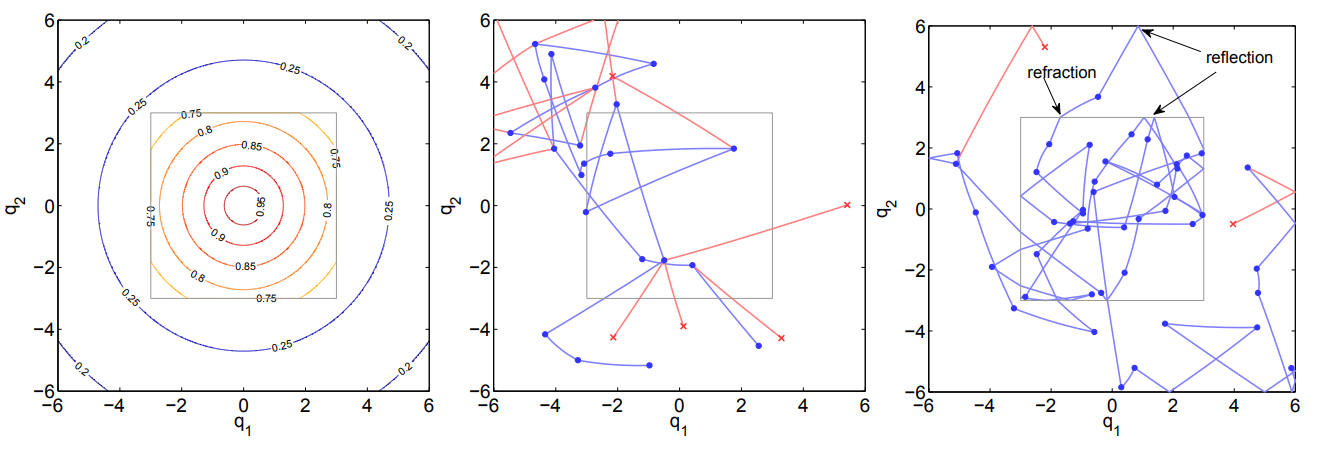
\includegraphics[width=0.9\textwidth]{publications/presentations/log_concave_sampling/reflection.png}
        \caption{Baseline and Reflective HMC. Taken from \cite{afshar2015reflection}.} 
        \label{fig:reflection}
    \end{figure}

\end{frame}

\begin{frame}[allowframebreaks]{The Reflection Operator}
    A point $x$ reflects at the boundary point $\tilde x$ with normal $n$.
    
    \medskip
    
    We define the reflection operator $\textrm{refl}$ such that 
    
    $$
    \textrm{refl}(x) = - 2 (a^T n) n + a + \tilde x
    $$

    where $a = \tilde x - x$ is the ray between the initial and the boundary points. Note that in general $\textrm{refl}(x)$ may not lie in $K$. We compose the reflection operator $k$ times such that $\textrm{refl}^k (x) = \mathrm {refl} \circ \dots \circ \mathrm{refl} (x) \in K$. In our setting we assume that at each step the proposal point cannot reflect more than $\ell \in \mathbb N^*$ times.

    \framebreak 
    
    \begin{figure}
        \centering
        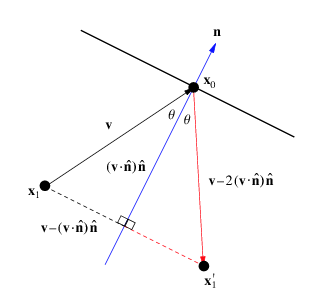
\includegraphics[width=0.4\textwidth]{publications/presentations/log_concave_sampling/reflection_w.png}
        \caption{Reflection Illustration. $x_1'$ is the reflection of $x_1$ about $x_0$ with normal $n$. Source: \url{https://mathworld.wolfram.com/Reflection.html}}
        \label{fig:my_label}
    \end{figure}
    
\end{frame}


\begin{frame}[allowframebreaks]{Computing Intersections with $\partial K$}
    
    
    Of particular interest is the computation of the intersection of an (implicit) curve between a point $x$ inside the convex body $K$ and a proposal $\tilde x \not \in K$. 
    
    \medskip

    \textbf{Case 1.} The curve is a \emph{line segment} and $K$ is a convex polytope.

    We parametrize the line segment between $x$ and $\tilde x$ with $\gamma(t) = t x + (1 - t) \tilde x$ where $t \in [0, 1]$. We seek $t_u = \sup \{ t \in [0, 1] | \gamma(t) \in \partial K \}$ and $u = \gamma(t_u)$ as the solution to the boundary intersection problem. 
    
    \medskip
    
    We use the Cyrus-Beck  \cite{cyrus1978generalized} algorithm
    
    \framebreak
    
    Let $z \in \partial K$ be known and let $n$ represent the normal vector at $z$. We compute the quantity 
    
    \begin{equation*}
        n^T (\gamma(t) - z) \begin{cases} = 0 & \gamma(t) \in \partial K \\
        < 0 & \gamma(t) \notin K \\
        > 0 & \gamma(t) \in K \setminus \partial K
        \end{cases}
    \end{equation*}

    Solving the equation $n^T (\gamma(t) - z)$ for $t$ we get 
    
    $$t = \frac {n^T (z - x)} {n^T (\tilde x - x)}$$

    We compute the above for all the $N$ normals of the polytope and keep the maximum value that lies in $[0, 1]$. The min value can also be kept in case we want the other intersetion point as well. Complexity is $O(Nd)$
    
    \framebreak
    
    \textbf{Case 2.} The curve has the form $\gamma(t) = \sum_{i = 1}^m a_i \phi_i(t)$, $\{ \phi_j \}_{j \in [m]}$ are basis functions, and $K$ is a convex polytope.
    
    \medskip
    
    We use the same procedure as above, however now we cannot solve directly for $t$. We, for example, can use the Newton-Raphson root finder to solve the transcendental equation.
    
    \begin{equation*}
        t^{(r + 1)} = t^{(r)} - \frac {\sum_{j \in [m]} (n^T a_j) \phi_j(t^{(r)}) - n^T z } {\sum_{j \in [m]} (n^T a_j) \dot \phi_j(t^{(r)})} \qquad r \in [R]
    \end{equation*}

    Complexity is $O(NdR)$ where $R$ is the maximum number of iterations the NR solver must be called to find a root. 
    
    \textbf{Problems.} Convergence, Well-posedness (denominator getting too small)

    \framebreak
    
    \textbf{Case 3.} The convex body $K$ has the form $K = \{ x \in \mathbb R^d | g(x) \le 0 \}$ where $g(x) = \max_{1 \le i \le M} g_i(x)$ where $g_1, \dots, g_M$ are twice-differentiable convex functions that are $\mu$-strongly-convex. 
    
    \medskip
    
    \textbf{Examples.} $L_2$ Balls, Spectrahedra etc.
    
    \medskip
    
    \textbf{Idea.} Linearize the convex body around $x + h$
    
    $$0 \ge g_i(x + h) \ge g_i(x) + \langle \nabla g_i(x), h \rangle + \frac {\mu \| h \|^2}  2 $$
    
    The linearized convex polytope $P(x)$ around $x$ is 
    
    $$J(x) h \le b$$
    
    where $J(x)$ is the Jacobian matrix around $x$ with entries $J_{ij}(x) = \frac {\partial g_i(x)} {\partial x_j}$ and $b$ has entries $b_i = -g_i(x)$.
    
    \framebreak 
    
    The linear approximation error is $O(\| h \|^2)$.     A high-level algorithm proceeds as follows.
    
    \medskip

    We are given a curve $\gamma(t)$ and a starting point $x_0 = \gamma(0)$, an accuracy $\epsilon > 0$, and a step counter $i$ initialized at 0.
    
    \begin{enumerate}
        
        \item Find $P(x_i)$ around $x_i$ and the intersection point of $\gamma(t)$ with $P(x_i)$ (see Case 1, Case 2). Let that point be $x_{i + 1} = \gamma(t_{i + 1})$
        \item Calculate $g(x_{i + 1}) = \max_{1 \le j \le M} g_j(x_{i + 1})$. If $|g(x_{i + 1)}| \le \epsilon$, output $x_{i + 1}, t_{i + 1}$, else repeat. 
    \end{enumerate}
    
    
    
\end{frame}

\begin{frame}{}
    \vfill
    \centering
    \Huge {
        \textbf{Thank you!}
    }
    \vfill
\end{frame}



\begin{frame}[allowframebreaks]{References}
    \small {

    \bibliographystyle{alpha}
    \bibliography{references}
    
    }
\end{frame}


\end{document}

